
\documentclass[letterpaper,hide notes,xcolor={table,svgnames},pdftex]{beamer}
\def\showexamples{t}


%\usepackage[svgnames]{xcolor}

%% Demo talk
%\documentclass[letterpaper,notes=show]{beamer}

\usecolortheme{crane}
\setbeamertemplate{navigation symbols}{}

\usetheme{MyPittsburgh}
%\usetheme{Frankfurt}

%\usepackage{tipa}

\usepackage{hyperref}
\usepackage{graphicx,xspace}
\usepackage[normalem]{ulem}

\newcommand\SF[1]{$\bigstar$\footnote{SF: #1}}



\newcounter{tmpnumSlide}
\newcounter{tmpnumNote}

% old question code
%\newcommand\question[1]{{$\bigstar$ \small \onlySlide{2}{#1}}}
% \newcommand\nquestion[1]{\ifdefined \presentationonly \textcircled{?} \fi \note{\par{\Large \textbf{?}} #1}}
% \newcommand\nanswer[1]{\note{\par{\Large \textbf{A}} #1}}


 \newcommand\mnote[1]{%
   \addtocounter{tmpnumSlide}{1}
   \ifdefined\showcues {~\tiny\fbox{\arabic{tmpnumSlide}}}\fi
   \note{\setlength{\parskip}{1ex}\addtocounter{tmpnumNote}{1}\textbf{\Large \arabic{tmpnumNote}:} {#1\par}}}

\newcommand\mmnote[1]{\note{\setlength{\parskip}{1ex}#1\par}}

%\newcommand\mnote[2][]{\ifdefined\handoutwithnotes {~\tiny\fbox{#1}}\fi
% \note{\setlength{\parskip}{1ex}\textbf{\Large #1:} #2\par}}

%\newcommand\mnote[2][]{{\tiny\fbox{#1}} \note{\setlength{\parskip}{1ex}\textbf{\Large #1:} #2\par}}

\newcommand\mquestion[2]{{~\color{red}\fbox{?}}\note{\setlength{\parskip}{1ex}\par{\Large \textbf{?}} #1} \note{\setlength{\parskip}{1ex}\par{\Large \textbf{A}} #2\par}\ifdefined \presentationonly \pause \fi}

\newcommand\blackboard[1]{%
\ifdefined   \showblackboard
  {#1}
  \else {\begin{center} \fbox{\colorbox{blue!30}{%
         \begin{minipage}{.95\linewidth}%
           \hspace{\stretch{1}} Some space intentionally left blank; done at the blackboard.%
         \end{minipage}}}\end{center}}%
         \fi%
}



%\newcommand\q{\tikz \node[thick,color=black,shape=circle]{?};}
%\newcommand\q{\ifdefined \presentationonly \textcircled{?} \fi}

\usepackage{listings}
\lstset{%
  keywordstyle=\bfseries,
  aboveskip=15pt,
  belowskip=15pt,
  captionpos=b,
  identifierstyle=\ttfamily,
  escapeinside={(*@}{@*)},
  stringstyle=\ttfamiliy,
  frame=lines,
  numbers=left, basicstyle=\scriptsize, numberstyle=\tiny, stepnumber=0, numbersep=2pt}

\usepackage{siunitx}
\newcommand\sius[1]{\num[group-separator = {,}]{#1}\si{\micro\second}}
\newcommand\sims[1]{\num[group-separator = {,}]{#1}\si{\milli\second}}
\newcommand\sins[1]{\num[group-separator = {,}]{#1}\si{\nano\second}}
\sisetup{group-separator = {,}, group-digits = true}

%% -------------------- tikz --------------------
\usepackage{tikz}
\usetikzlibrary{positioning}
\usetikzlibrary{arrows,backgrounds,automata,decorations.shapes,decorations.pathmorphing,decorations.markings,decorations.text}

\tikzstyle{place}=[circle,draw=blue!50,fill=blue!20,thick, inner sep=0pt,minimum size=6mm]
\tikzstyle{transition}=[rectangle,draw=black!50,fill=black!20,thick, inner sep=0pt,minimum size=4mm]

\tikzstyle{block}=[rectangle,draw=black, thick, inner sep=5pt]
\tikzstyle{bullet}=[circle,draw=black, fill=black, thin, inner sep=2pt]

\tikzstyle{pre}=[<-,shorten <=1pt,>=stealth',semithick]
\tikzstyle{post}=[->,shorten >=1pt,>=stealth',semithick]
\tikzstyle{bi}=[<->,shorten >=1pt,shorten <=1pt, >=stealth',semithick]

\tikzstyle{mut}=[-,>=stealth',semithick]

\tikzstyle{treereset}=[dashed,->, shorten >=1pt,>=stealth',thin]

\usepackage{ifmtarg}
\usepackage{xifthen}
\makeatletter
% new counter to now which frame it is within the sequence
\newcounter{multiframecounter}
% initialize buffer for previously used frame title
\gdef\lastframetitle{\textit{undefined}}
% new environment for a multi-frame
\newenvironment{multiframe}[1][]{%
\ifthenelse{\isempty{#1}}{%
% if no frame title was set via optional parameter,
% only increase sequence counter by 1
\addtocounter{multiframecounter}{1}%
}{%
% new frame title has been provided, thus
% reset sequence counter to 1 and buffer frame title for later use
\setcounter{multiframecounter}{1}%
\gdef\lastframetitle{#1}%
}%
% start conventional frame environment and
% automatically set frame title followed by sequence counter
\begin{frame}%
\frametitle{\lastframetitle~{\normalfont(\arabic{multiframecounter})}}%
}{%
\end{frame}%
}
\makeatother

\makeatletter
\newdimen\tu@tmpa%
\newdimen\ydiffl%
\newdimen\xdiffl%
\newcommand\ydiff[2]{%
    \coordinate (tmpnamea) at (#1);%
    \coordinate (tmpnameb) at (#2);%
    \pgfextracty{\tu@tmpa}{\pgfpointanchor{tmpnamea}{center}}%
    \pgfextracty{\ydiffl}{\pgfpointanchor{tmpnameb}{center}}%
    \advance\ydiffl by -\tu@tmpa%
}
\newcommand\xdiff[2]{%
    \coordinate (tmpnamea) at (#1);%
    \coordinate (tmpnameb) at (#2);%
    \pgfextractx{\tu@tmpa}{\pgfpointanchor{tmpnamea}{center}}%
    \pgfextractx{\xdiffl}{\pgfpointanchor{tmpnameb}{center}}%
    \advance\xdiffl by -\tu@tmpa%
}
\makeatother
\newcommand{\copyrightbox}[3][r]{%
\begin{tikzpicture}%
\node[inner sep=0pt,minimum size=2em](ciimage){#2};
\usefont{OT1}{phv}{n}{n}\fontsize{4}{4}\selectfont
\ydiff{ciimage.south}{ciimage.north}
\xdiff{ciimage.west}{ciimage.east}
\ifthenelse{\equal{#1}{r}}{%
\node[inner sep=0pt,right=1ex of ciimage.south east,anchor=north west,rotate=90]%
{\raggedleft\color{black!50}\parbox{\the\ydiffl}{\raggedright{}#3}};%
}{%
\ifthenelse{\equal{#1}{l}}{%
\node[inner sep=0pt,right=1ex of ciimage.south west,anchor=south west,rotate=90]%
{\raggedleft\color{black!50}\parbox{\the\ydiffl}{\raggedright{}#3}};%
}{%
\node[inner sep=0pt,below=1ex of ciimage.south west,anchor=north west]%
{\raggedleft\color{black!50}\parbox{\the\xdiffl}{\raggedright{}#3}};%
}
}
\end{tikzpicture}
}


%% --------------------

%\usepackage[excludeor]{everyhook}
%\PushPreHook{par}{\setbox0=\lastbox\llap{MUH}}\box0}

%\vspace*{\stretch{1}

%\setbox0=\lastbox \llap{\textbullet\enskip}\box0}

\setlength{\parskip}{\fill}

\newcommand\noskips{\setlength{\parskip}{1ex}}
\newcommand\doskips{\setlength{\parskip}{\fill}}

\newcommand\xx{\par\vspace*{\stretch{1}}\par}
\newcommand\xxs{\par\vspace*{2ex}\par}
\newcommand\tuple[1]{\langle #1 \rangle}
\newcommand\code[1]{{\sf \footnotesize #1}}
\newcommand\ex[1]{\uline{Example:} \ifdefined \presentationonly \pause \fi
  \ifdefined\showexamples#1\xspace\else{\uline{\hspace*{2cm}}}\fi}

\newcommand\ceil[1]{\lceil #1 \rceil}


\AtBeginSection[]
{
   \begin{frame}
       \frametitle{Outline}
       \tableofcontents[currentsection]
   \end{frame}
}



\pgfdeclarelayer{edgelayer}
\pgfdeclarelayer{nodelayer}
\pgfsetlayers{edgelayer,nodelayer,main}

\tikzstyle{none}=[inner sep=0pt]
\tikzstyle{rn}=[circle,fill=Red,draw=Black,line width=0.8 pt]
\tikzstyle{gn}=[circle,fill=Lime,draw=Black,line width=0.8 pt]
\tikzstyle{yn}=[circle,fill=Yellow,draw=Black,line width=0.8 pt]
\tikzstyle{empty}=[circle,fill=White,draw=Black]
\tikzstyle{bw} = [rectangle, draw, fill=blue!20, 
    text width=4em, text centered, rounded corners, minimum height=2em]
    
    \newcommand{\CcNote}[1]{% longname
	This work is licensed under the \textit{Creative Commons #1 3.0 License}.%
}
\newcommand{\CcImageBy}[1]{%
	\includegraphics[scale=#1]{creative_commons/cc_by_30.pdf}%
}
\newcommand{\CcImageSa}[1]{%
	\includegraphics[scale=#1]{creative_commons/cc_sa_30.pdf}%
}
\newcommand{\CcImageNc}[1]{%
	\includegraphics[scale=#1]{creative_commons/cc_nc_30.pdf}%
}
\newcommand{\CcGroupBySa}[2]{% zoom, gap
	\CcImageBy{#1}\hspace*{#2}\CcImageNc{#1}\hspace*{#2}\CcImageSa{#1}%
}
\newcommand{\CcLongnameByNcSa}{Attribution-NonCommercial-ShareAlike}

\newenvironment{changemargin}[1]{% 
  \begin{list}{}{% 
    \setlength{\topsep}{0pt}% 
    \setlength{\leftmargin}{#1}% 
    \setlength{\rightmargin}{1em}
    \setlength{\listparindent}{\parindent}% 
    \setlength{\itemindent}{\parindent}% 
    \setlength{\parsep}{\parskip}% 
  }% 
  \item[]}{\end{list}} 




\title{Lecture 32 --- Software Architecture Patterns}

\author{Jeff Zarnett \\ \small \texttt{jzarnett@uwaterloo.ca}}
\institute{Department of Electrical and Computer Engineering \\
  University of Waterloo}
\date{\today}


\begin{document}

\begin{frame}
  \titlepage
\end{frame}

\begin{frame}
\frametitle{Software Architecture Pattern}

\begin{changemargin}{1cm}
Software Architecture Pattern: a general, re-usable solution for how to structure software.

At a high level, nearly all software has three major elements:

\begin{enumerate}
	\item Logic \mnote{the software does some work}
	\item Data \mnote{it stores and/or retrieves some data somehow, and}
	\item User Interface \mnote{it presents information to and accepts information and/or commands from the user or users.}
\end{enumerate}

\end{changemargin}
\end{frame}

\begin{frame}
\frametitle{Software Architecture Patterns}

\begin{changemargin}{1cm}
Different patterns apply to different problems.

Large software almost never has exactly 1 architecture pattern.


Different patterns used in different parts of the same program.

Some deviation from the pattern is normal.

\end{changemargin}
\end{frame}



\begin{frame}
\frametitle{Architecture Patterns: Motivation}

\begin{changemargin}{1cm}
Similar to why we use life cycle models.

In university assignments, you can get away without structure.\\
\quad This tends to result in the ``monolith'' pattern.

Bigger software will require deliberate choices of architecture.\\
\quad Otherwise, a mess to clean up later.

\end{changemargin}
\end{frame}

\begin{frame}
\frametitle{Architecture Patterns: Monolith}

\begin{changemargin}{1cm}
The monolith is a single, self-contained program.

No defined modules, no clear lines between different parts.

Logic, user interface, and data all mixed together.

Probably your university work looks like this.

\end{changemargin}
\end{frame}


\begin{frame}
\frametitle{Architecture Patterns: Monolith}

\begin{changemargin}{1cm}
Mainframe applications used to be written like this.

Complexity spirals out of control.

Eventually becomes unmaintainable.


\end{changemargin}
\end{frame}

\begin{frame}
\frametitle{Architecture Patterns: Monolith}

\begin{changemargin}{1cm}

Often faster to write than other structures.

Tradeoff: more difficult to understand and maintain.

Changes might have unexpected consequences.

Not necessarily the wrong choice: see Microsoft Word.


\end{changemargin}
\end{frame}


\begin{frame}
\frametitle{Architecture Patterns: Client-Server}


\begin{center}
	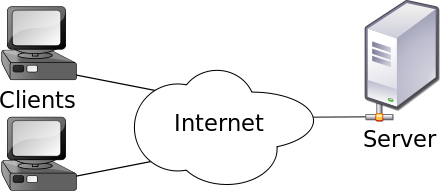
\includegraphics[width=0.7\textwidth]{images/Client-server-model.png}
	
	\texttt{\small
 http://en.wikipedia.org/wiki/File:Client-server-model.svg}
\end{center}

Two roles: client and server.

\end{frame}

\begin{frame}
\frametitle{Architecture Patterns: Client-Server}

\begin{changemargin}{1cm}

Client and Server communicate via a request-response pattern.

Client sends requests; server sends responses.

The two must understand each other. Protocol.

Examples: E-mail, World Wide Web, Banking

\end{changemargin}
\end{frame}


\begin{frame}
\frametitle{Architecture Patterns: Client-Server}

\begin{changemargin}{1cm}

There is a clear line dividing client and server.

Most often, logic and data are on the server; client handles UI.

Often client \& server on different physical machines.\\
\quad But this is not a requirement.

\end{changemargin}
\end{frame}

\begin{frame}
\frametitle{Architecture Patterns: Client-Server}

\begin{changemargin}{1cm}

Example: opening a web page, \texttt{www.google.com}.

Browser sends request to Google. Google server responds.

The browser does not know or care how the server generates its answer.

The server does not know or care how the request was generated, or how the browser draws the response page.

\end{changemargin}
\end{frame}

\begin{frame}
\frametitle{Architecture Patterns: Client-Server}

\begin{changemargin}{1cm}
Historical Note: Mainframes and Batch Jobs

At one time, lots of computing used client-server.

PCs were expensive and mainframes were common. 

Desk computers were ``thin clients'' or ``dumb terminals'';\\
\quad Little or no processing power of their own.\\
\quad Sent work to the server and displayed responses.


\end{changemargin}
\end{frame}

\begin{frame}
\frametitle{Architecture Patterns: Client-Server}

\begin{changemargin}{1cm}
Mainframes and Batch Job Example

When programming, the programmer edits code on her PC.

To compile, submit a \textit{batch job} -- server request.

Server takes the code, compiles it, and returns the result.

\end{changemargin}
\end{frame}

\begin{frame}
\frametitle{Architecture Patterns: Client-Server}

\begin{changemargin}{1cm}
Batch Job processing is uncommon now.

PC prices fell and their power increased (starting in the 80s).

More efficient to buy powerful PCs; have them do the work.

Compiling is now done on local machines.\\
\quad Although there are often official build servers.

\end{changemargin}
\end{frame}

\begin{frame}
\frametitle{Architecture Patterns: Client-Server}

\begin{changemargin}{1cm}
Typically possible to replace either the client or server\\
\quad ...as long as the communication protocol is unchanged.

Example: we can access Google with Firefox or Chrome.

Advantage over monolith: separated concerns.

Risk: central server crash might stop the whole system! \mnote{Aside: some people may attempt to cause a server crash with the explicit intent of denying all other users access to the server, but we'll talk about security later on in the term.}

\end{changemargin}
\end{frame}

\begin{frame}
\frametitle{Architecture Patterns: Three-Tier}

\begin{center}
	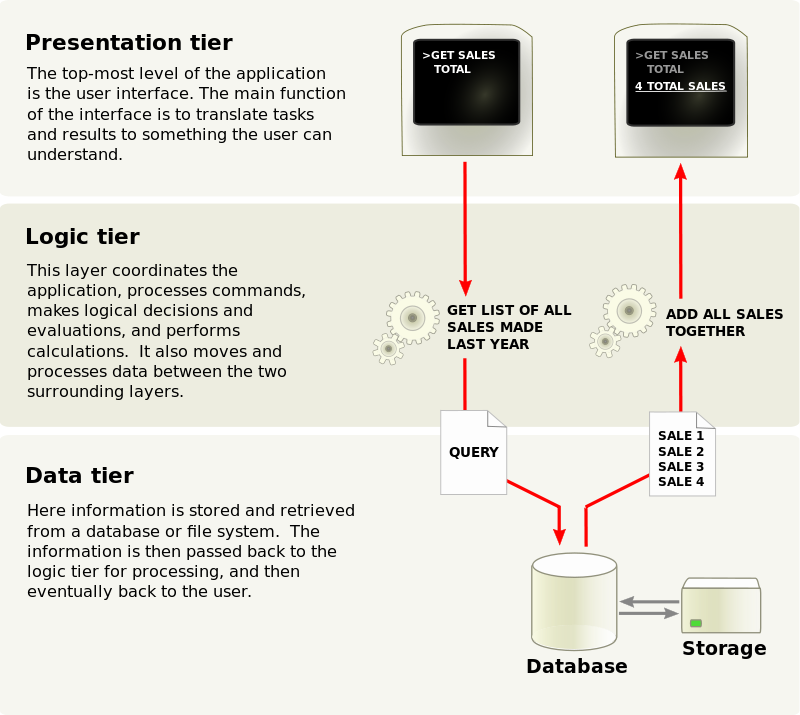
\includegraphics[width=0.7\textwidth]{images/threetier.png}
	
	\texttt{\tiny
 http://en.wikipedia.org/wiki/File:Overview\_of\_a\_three-tier\_application\_vectorVersion.svg}
\end{center}

\end{frame}

\begin{frame}
\frametitle{Architecture Patterns: Three-Tier}

\begin{changemargin}{1cm}
Consists of three distinct but interacting parts.

The user interface, logic, and data reside in their own areas.

These can be separate physical systems, but don't have to be.

\end{changemargin}
\end{frame}

\begin{frame}
\frametitle{Architecture Patterns: Three-Tier}

\begin{changemargin}{1cm}
Each tier can be changed without affecting the other parts.

Example: present data on Android and not just Windows.

Example 2: change database from mySQL to Oracle.

Tiers can be subdivided further, especially the logic tier.\\
\quad Then we have an \textit{n-Tier} architecture.


\end{changemargin}
\end{frame}

\begin{frame}
\frametitle{Architecture Patterns: Three-Tier}

Let's examine the tier descriptions more closely.

\begin{center}
	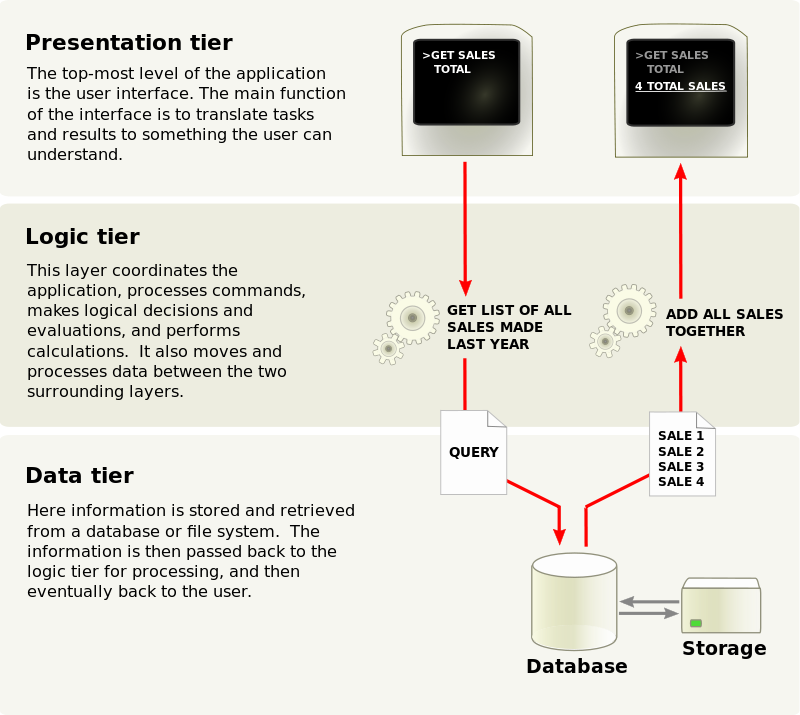
\includegraphics[width=0.65\textwidth]{images/threetier.png}
	
	\texttt{\tiny
 http://en.wikipedia.org/wiki/File:Overview\_of\_a\_three-tier\_application\_vectorVersion.svg}
\end{center}

\end{frame}

\begin{frame}
\frametitle{Architecture Patterns: Three-Tier}

\begin{changemargin}{1cm}
Can be used in combination with client-server model.

Most common split: client has UI, server has logic and data.

Note that the client can have logic of its own\\
\quad So the dividing line could be anywhere in the logic tier.

Presentation tier does not communicate with the data tier.\\
\quad Communication only between adjacent tiers.

\end{changemargin}
\end{frame}

\begin{frame}
\frametitle{Architecture Patterns: Three-Tier}

\begin{changemargin}{1cm}
Client-Server interaction can occur between any \textit{adjacent} tiers.

Obvious case: presentation tier a client to logic tier's server.

From the perspective of the data tier: data tier is the server, responding to requests from a client, the logic tier.

\end{changemargin}
\end{frame}

\begin{frame}
\frametitle{Architecture Patterns: Three-Tier}

\begin{changemargin}{1cm}
Revisit the Google example. This time we'll search!

The browser remains the presentation tier in this example.

\begin{enumerate}
\item Browser sends to the server our search request. 

\item The server analyzes our request and queries the database for matches on these search terms. 

\item The database returns the results to the logic tier.

\item The logic tier formats the results into a webpage. 

\item The logic tier sends the answer back to your browser. 

\item The browser draws the page on the screen.
\end{enumerate}

\end{changemargin}
\end{frame}



\begin{frame}
\frametitle{Architecture Patterns: Model-View-Controller}
\begin{center}

	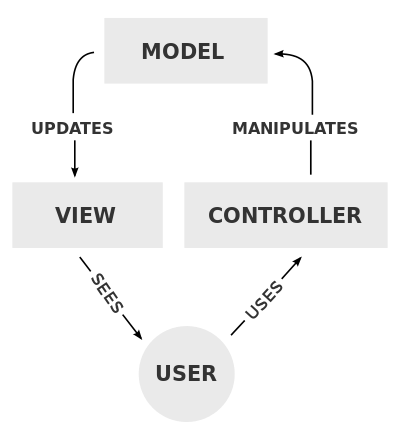
\includegraphics[width=0.5\textwidth]{images/mvc.png}
	
	\texttt{\small http://en.wikipedia.org/wiki/File:MVC-Process.svg}
\end{center}
\end{frame}

\begin{frame}
\frametitle{Architecture Patterns: Model-View-Controller}

\begin{changemargin}{1cm}
Model-View-Controller is often abbreviated MVC.

Software is divided into the model, view, and controller.

The pattern also defines the interactions of these three.

\end{changemargin}
\end{frame}

\begin{frame}
\frametitle{Architecture Patterns: Model-View-Controller}

\begin{changemargin}{1cm}
Model-View-Controller is often abbreviated MVC.

Software is divided into the model, view, and controller.

The pattern also defines the interactions of these three.

Example: \texttt{Contact} object, holding contact info for a person or business (e.g., phone number)

\end{changemargin}
\end{frame}

\begin{frame}
\frametitle{Architecture Patterns: Model-View-Controller}

\begin{changemargin}{1cm}
The Model:
\begin{itemize}
	\item Holds a reference to the \texttt{Contact}
	\item Contains business logic and functions.
	\item Notifies view(s) and controller(s) of changes to \texttt{Contact}
	\item View, Controller must use model to access \texttt{Contact}
\end{itemize}

\end{changemargin}
\end{frame}

\begin{frame}
\frametitle{Architecture Patterns: Model-View-Controller}

\begin{changemargin}{1cm}
The View:
\begin{itemize}
	\item Any representation of \texttt{Contact} data.
	\item We can have multiple views of the same data.
	\item Requests from the model info it needs to display.
\end{itemize}

\end{changemargin}
\end{frame}


\begin{frame}
\frametitle{Architecture Patterns: Model-View-Controller}

\begin{changemargin}{1cm}
The Controller:
\begin{itemize}
	\item Accepts input; converts it to commands.
	\item Commands sent to model manipulate data.
	\item Commands sent to view change the view (e.g. scrolling).
\end{itemize}

\end{changemargin}
\end{frame}

\begin{frame}
\frametitle{Architecture Patterns: Model-View-Controller}

\begin{changemargin}{1cm}
MVC Example.

User wants to set phone number to null.

Clicks on button ``Clear Phone Number''.

The click is input to the controller.

Controller turns this into a command for the model:\\
	\quad \texttt{setPhoneNumber(null);}

\end{changemargin}
\end{frame}

\begin{frame}
\frametitle{Architecture Patterns: Model-View-Controller}

\begin{changemargin}{1cm}
MVC Example Continued.

Model executes command - \texttt{Contact} is updated.

Model notifies the view that the \texttt{Contact} has changed.

View re-draws the screen to reflect the change.
\end{changemargin}
\end{frame}


\begin{frame}
\frametitle{Architecture Patterns: Model-View-Controller}
\begin{center}

	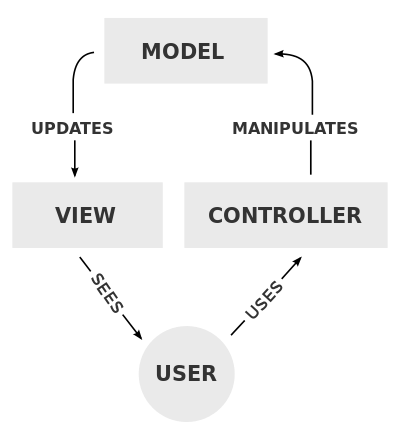
\includegraphics[width=0.5\textwidth]{images/mvc.png}
	
	\texttt{\small http://en.wikipedia.org/wiki/File:MVC-Process.svg}
\end{center}
\end{frame}


\begin{frame}
\frametitle{Architecture Patterns: Model-View-Controller}

\begin{changemargin}{1cm}
Considered good practice because it separates logic from UI.

We can have different ways of viewing the data. \mnote{full screen or mobile screen}

One element (often the view) can be changed without affecting others.
\end{changemargin}
\end{frame}

\begin{frame}
\frametitle{Architecture Patterns: Model-View-Controller}

\begin{changemargin}{1cm}
MVC overlaps with client-server.

The client might call up a record from the server and then use MVC for the user to manipulate it, 

One of the model actions is save changes\\
\quad (send them back to the server for storage). 

Thin-client system: the client has the view and controller; server has the model.

\end{changemargin}
\end{frame}

\begin{frame}
\frametitle{Architecture Patterns: Model-View-Controller}

\begin{changemargin}{1cm}
MVC overlaps with three tier as well.

The view and controller are presentation tier \\
\quad model in the logic tier.

MVC, Three-Tier, and Client-Server can all work together. \mnote{One way this might happen is the client has the view and controller (presentation tier), the server has the model (logic tier), and the objects represented, such as the \texttt{Contact} described earlier, is stored in the data tier (also on the server side).}

\end{changemargin}
\end{frame}

\begin{frame}
\frametitle{Architecture Patterns: Modular Architecture}
\begin{center}
	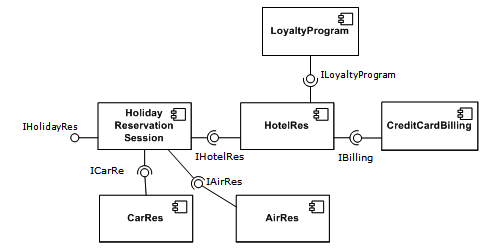
\includegraphics[width=\textwidth]{images/cbse.png}
	
	\texttt{\tiny
http://en.wikipedia.org/wiki/File:Component-based-Software-Engineering-example2.gif}
\end{center}
\end{frame}

\begin{frame}
\frametitle{Architecture Patterns: Modular Architecture}

\begin{changemargin}{1cm}
As defined so far, the client and server (or tiers) might themselves be described as being monolithic.

One or both of those might be too complex for monolith.

Solution: modules!

The final software product is comprised of a number of modules which interact.

A module, sometimes called a component, contains a related set of methods/functions or data. 

The modular architecture is also sometimes called ``Component-Based Software Engineering''.

\end{changemargin}
\end{frame}

\begin{frame}
\frametitle{Architecture Patterns: Modular Architecture}
\begin{center}
	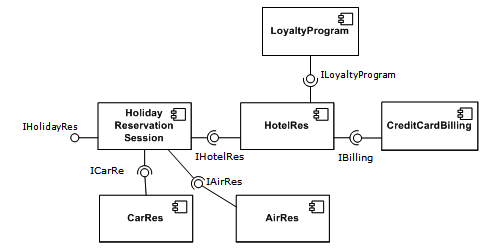
\includegraphics[width=\textwidth]{images/cbse.png}
	
	\texttt{\tiny
http://en.wikipedia.org/wiki/File:Component-based-Software-Engineering-example2.gif}
\end{center}
\end{frame}

\begin{frame}
\frametitle{Architecture Patterns: Modular Architecture}

\begin{changemargin}{1cm}
The distinct boxes indicate that parts can be swapped in and out.

If the loyalty program moves to a new airline, swap \texttt{AirRes} without changing anything else.

Under ideal circumstances, components can be re-used. \mnote{If the company running the loyalty program decided to expand its business by opening up a rewards shop, where you could buy items online. If the credit card billing module is implemented well, that component can be re-used, without changes, in the online store system. 
}
\end{changemargin}
\end{frame}


\end{document}
